% !TEX TS-program = pdflatex
% !TEX encoding = UTF-8 Unicode

\documentclass[a4paper, titlepage=false, parskip=full-, 10pt]{scrartcl}

\usepackage[utf8]{inputenc}
\usepackage[T1]{fontenc}
\usepackage[english, ngerman]{babel}
\usepackage{babelbib}
\usepackage{hyperref}
\usepackage{listings}
\usepackage{framed}
\usepackage{color}
\usepackage{graphicx}
\usepackage[normalem]{ulem}
\usepackage{cancel}
\usepackage{amsmath}
\usepackage{amssymb}
\usepackage{amsthm}
\usepackage{algorithm}
\usepackage{algorithmic}
\usepackage{geometry}
\usepackage{subfigure}
\geometry{a4paper, top=20mm, left=35mm, right=25mm, bottom=40mm}

\newcounter{tasknbr}
\setcounter{tasknbr}{1}
\newenvironment{task}[1]{{\bf Aufgabe \arabic {tasknbr}\stepcounter{tasknbr}} (#1):\begin{enumerate}}{\end{enumerate}}
\newcommand{\subtask}[1]{\item[#1)]}

% Listings -----------------------------------------------------------------------------
\definecolor{red}{rgb}{.8,.1,.2}
\definecolor{blue}{rgb}{.2,.3,.7}
\definecolor{lightyellow}{rgb}{1.,1.,.97}
\definecolor{gray}{rgb}{.7,.7,.7}
\definecolor{darkgreen}{rgb}{0,.5,.1}
\definecolor{darkyellow}{rgb}{1.,.7,.3}
\lstloadlanguages{C++,[Objective]C,Java}
\lstset{
escapeinside={§§}{§§},
basicstyle=\ttfamily\footnotesize\mdseries,
columns=fullflexible, % typewriter font look better with fullflex
keywordstyle=\bfseries\color{blue},
% identifierstyle=\bfseries,
commentstyle=\color{darkgreen},      
stringstyle=\color{red},
numbers=left,
numberstyle=\ttfamily\scriptsize\color{gray},
% stepnumber=5,
% numberfirstline=true,
breaklines=true,
% prebreak=\\,
showstringspaces=false,
tabsize=4,
captionpos=b,
% framexrightmargin=-.2\textwidth,
float=htb,
frame=tb,
frameshape={RYR}{y}{y}{RYR},
rulecolor=\color{black},
xleftmargin=15pt,
xrightmargin=4pt,
aboveskip=\bigskipamount,
belowskip=\bigskipamount,
backgroundcolor=\color{lightyellow},
extendedchars=true,
belowcaptionskip=15pt}

%% Enter current values here: %%
\newcommand{\lecture}{Algorithmische Geometrie SS15}
\newcommand{\tutor}{}
\newcommand{\assignmentnbr}{7}
\newcommand{\students}{Julius Auer, Alexa Schlegel}
%%-------------------------------------%%

\begin{document}  
{\small \textsl{\lecture \hfill \tutor}}
\hrule
\begin{center}
\textbf{Übungsblatt \assignmentnbr}\\
[\bigskipamount]
{\small \students}
\end{center}
\hrule

\begin{task}{Anfragezeit bei kd-Bäumen}
\item[]
Die Argumentation ist die Selbe wie für $k=2$:\\
(1) Seien für einen Knoten $v$, dessen Region $R_v$ und eine Suchregion $U$ mit einer beliebigen, festen Kante $L$ zunächst $R_v\cap L\ne\emptyset$. Für $k=2$ war zu beobachten, dass von den 4 primären Enkelregionen von $v$ maximal 2 von $L$ geschnitten werden können. Diese Beobachtung lässt sich alternativ auch so interpretieren, dass in der Dimension in der $L$ eine Kante ist, auf jeden Fall ein Kind nicht betrachtet wird. Auch für $k>2$ wird in dieser einen Dimension ein Kind nicht betrachtet - in allen $k-1$ anderen können beide Pfade im Baum verfolgt werden. Die Rekursion für die Anzahl besuchter Primärknoten $p_s$ in Tiefe $s$ ergibt sich somit zu:
$$p_{s+k}\le 2\cdot (k-1)\cdot p_s$$
mit $k-1$ Rekursionsankern. Für $k=2$ und $k=3$ erhält man exemplarisch:
\begin{align*}
p_0&=1&p_0&=1\\
p_2&\le 2&p_3&\le 4\\
p_4&\le 4&p_6&\le 16\\
p_6&\le 8&p_9&\le 64\\
p_8&\le 16&p_{12}&\le 256\\
...&&...\\
p_s&\le 2^{\lceil\frac{s}{2}\rceil}&p_s&\le 2^{\lceil\frac{2}{3}\cdot s \rceil}
\end{align*} 
Oder im Allgemeinen für beliebiges $k$:
$$p_s\le 2^{\lceil\left(1-\frac{1}{k}\right)\cdot s \rceil}$$
Diese Beobachtung verbleibt - wie auch in der Vorlesung im Fall $k=2$ gesehen - ohne Beweis.

Alles Weitere verhält sich wie für den Fall $k=2$ in der Vorlesung betrachtet und sei im Folgenden nur kurz zusammengefasst:

Neben dem oben geschilderten Fall können noch zwei weitere auftreten:

(2) $R_v\subset U$: ist durch $O(m)$ abgedeckt.

(3) Suchen in einem $=$-Teilbaum benötigt höchstens (wenn die Region nicht ganz in $L$ liegt) $2\cdot (\log n-s)$ Schritte.

Somit erhält man insgesamt für die Anzahl besuchter Knoten:
\begin{align*}
=&\sum_{s=0}^{\lceil\log n\rceil}\overbrace{2^{\lceil 1-\frac{1}{k}\rceil\cdot s}}^{(1)}\cdot\left(\overbrace{1}^{v}+\overbrace{2\cdot (\log n-s)}^{(3)}\right)\\
\le&2\cdot\sum_{s=0}^{(\log n)+1}2^{(1-\frac{1}{k})\cdot s}\cdot (1+2\cdot (\log n-s))\\
=&2\cdot\sum_{s=0}^{(\log n)+1}\left(2^{1-\frac{1}{k}}\right)^{\log n}\cdot\frac{\left(2^{1-\frac{1}{k}}\right)^s}{\left(2^{1-\frac{1}{k}}\right)^{\log n}}\cdot (1+2\cdot (\log n-s))\\
=&2\cdot n^{1-\frac{1}{k}}\cdot\sum_{s=0}^{(\log n)+1}\left(2^{1-\frac{1}{k}}\right)^{s-\log n}\cdot (1+2\cdot (\log n-s))\\
=&2\cdot n^{1-\frac{1}{k}}\cdot\sum_{s=0}^{(\log n)+1}\frac{1+2\cdot (\log n-s)}{\left(2^{1-\frac{1}{k}}\right)^{\log n-s}}
\end{align*}
Der Term in der Summe konvergiert und unter Berücksichtigung von (2) ergibt sich die Anzahl ingesamt besuchter Knoten zu:
$$O\left(n^{1-\frac{1}{k}}+m\right)$$
\end{task}

\begin{task}{Implementierung}
\item[]
Zum Ausführen des Codes muss bitte \emph{orte\_deutschland.txt} im selben Verzeichnis wie das Jar liegen, oder wahlweise das Jar mit Angabe des Pfads gestartet werden:\\
\emph{java -jar AlGeo.jar <path>/orte\_deutschland.txt}

Um einen kd-Baum in $O(n\cdot (k+\log n))$ konstruieren zu können, benötigt man einen $O(n)$-Median Algorithmus. Wir haben zu diesem Zweck der Vollständigkeit halber einen \emph{BFPRT} implementiert - dieser ist in der Praxis aber deutlich langsamer als das mittlere Element nach Sortieren mit \emph{Timsort} zu ermitteln. Deshalb wird für den kd-Baum letztgenannter Ansatz verwendet. 

Da für das Erstellen eines ausgeglichenen kd-Baums alle Elemente zur Konstruktions-Zeit bekannt sein müssen, wurde auf eine \emph{insert}-Methode verzichtet.

Der kd-Baum akzeptiert als Elemente alle Objekte, die \emph{KDKey} implementieren - über diese Schnittstelle kann für jedes Objekt auf das $i$-te Element des $k$-dimensionalen Schlüssels zugegriffen werden:

\lstinputlisting[language=Java, firstline=3]{../../AlGeo/src/kdtrees/KDKey.java}

Alle übrigen Details sollten den Kommentaren zu entnehmen sein. Es folgt der vollständige Code:

\lstinputlisting[language=Java, firstline=6]{../../AlGeo/src/kdtrees/KDTree.java}
\lstinputlisting[language=Java, firstline=8]{../../AlGeo/src/kdtrees/Node.java}

Ein Test mit der großen \emph{orte\_welt.txt}-Datei wurde nicht durchgeführt, weil der File das Filesize-Limit von Github überschreitet - damit passt er nicht in unseren Workflow :)

Für deutsche Orte wurden alle Orte als schwarze Punkte eingezeichnet und die Orte aus der Ergebnismenge von Beispiel-Anfragen (markiert durch rote Boxen um den Anfrage-Bereich) als grüne Punkte (Abb. \ref{fig:2.1}).

\begin{figure}[h!]
\begin{center}
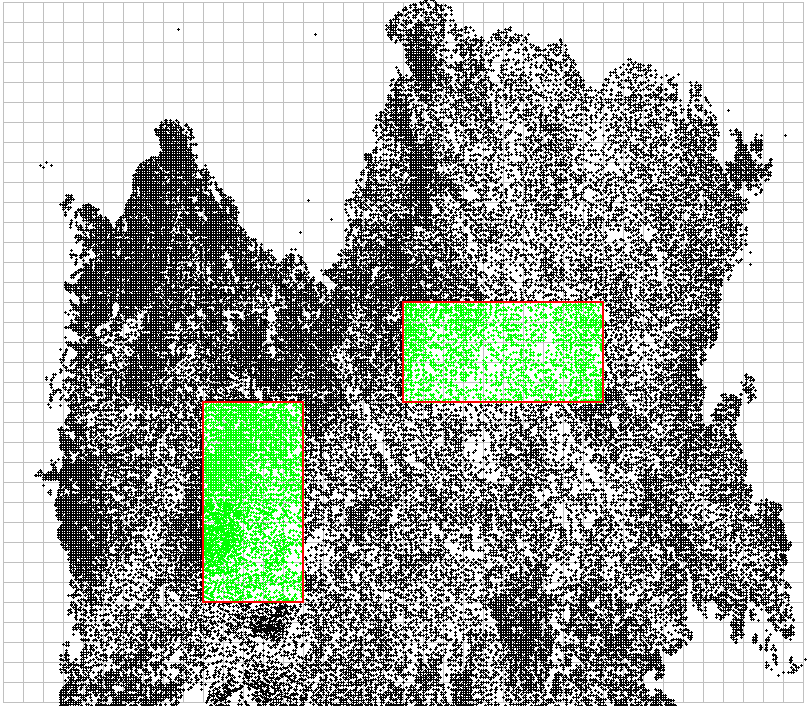
\includegraphics[width=8cm]{capture1}
\end{center}
\caption{Zwei Beispielanfragen}
\label{fig:2.1}
\end{figure}
\end{task}
\end{document}